\begin{figure}[H]
  \centering
  \begin{subfigure}[b]{.5\textwidth}
    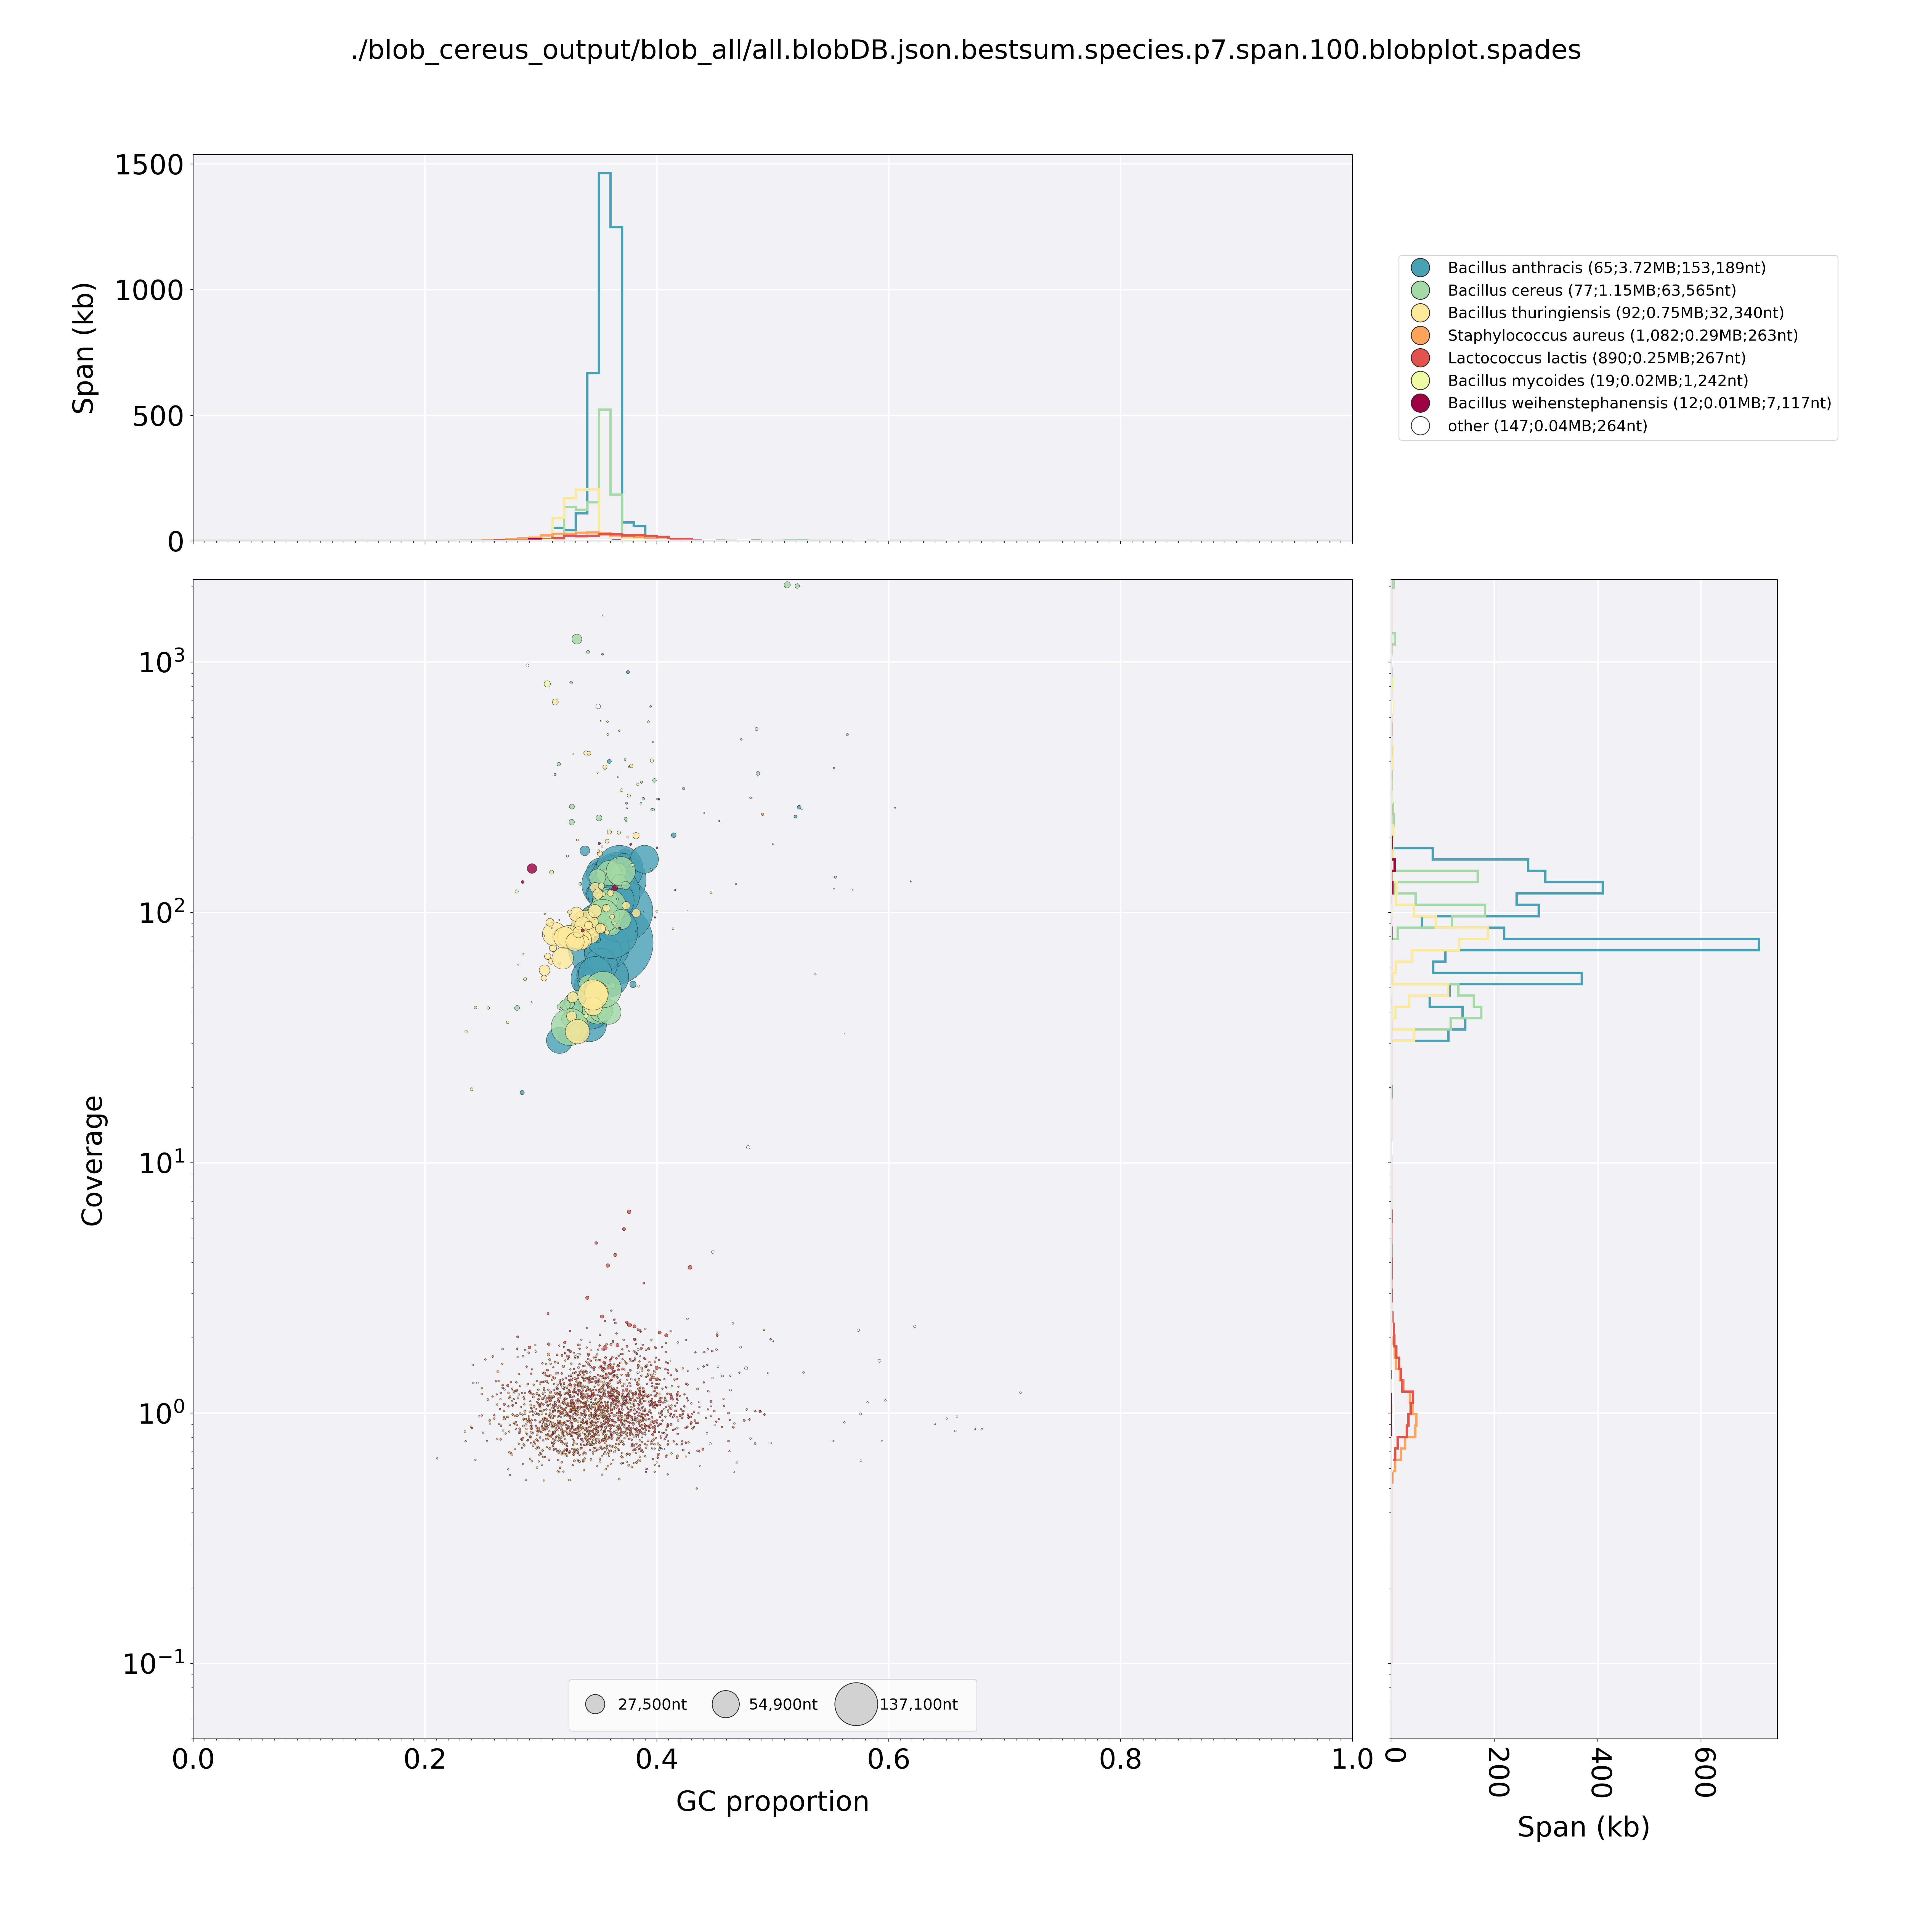
\includegraphics[width=.95\textwidth]{all.blobDB.json.bestsum.species.p7.span.100.blobplot.spades.png}
    \caption{All reads}
  \end{subfigure}
  \begin{subfigure}[b]{.5\textwidth}
    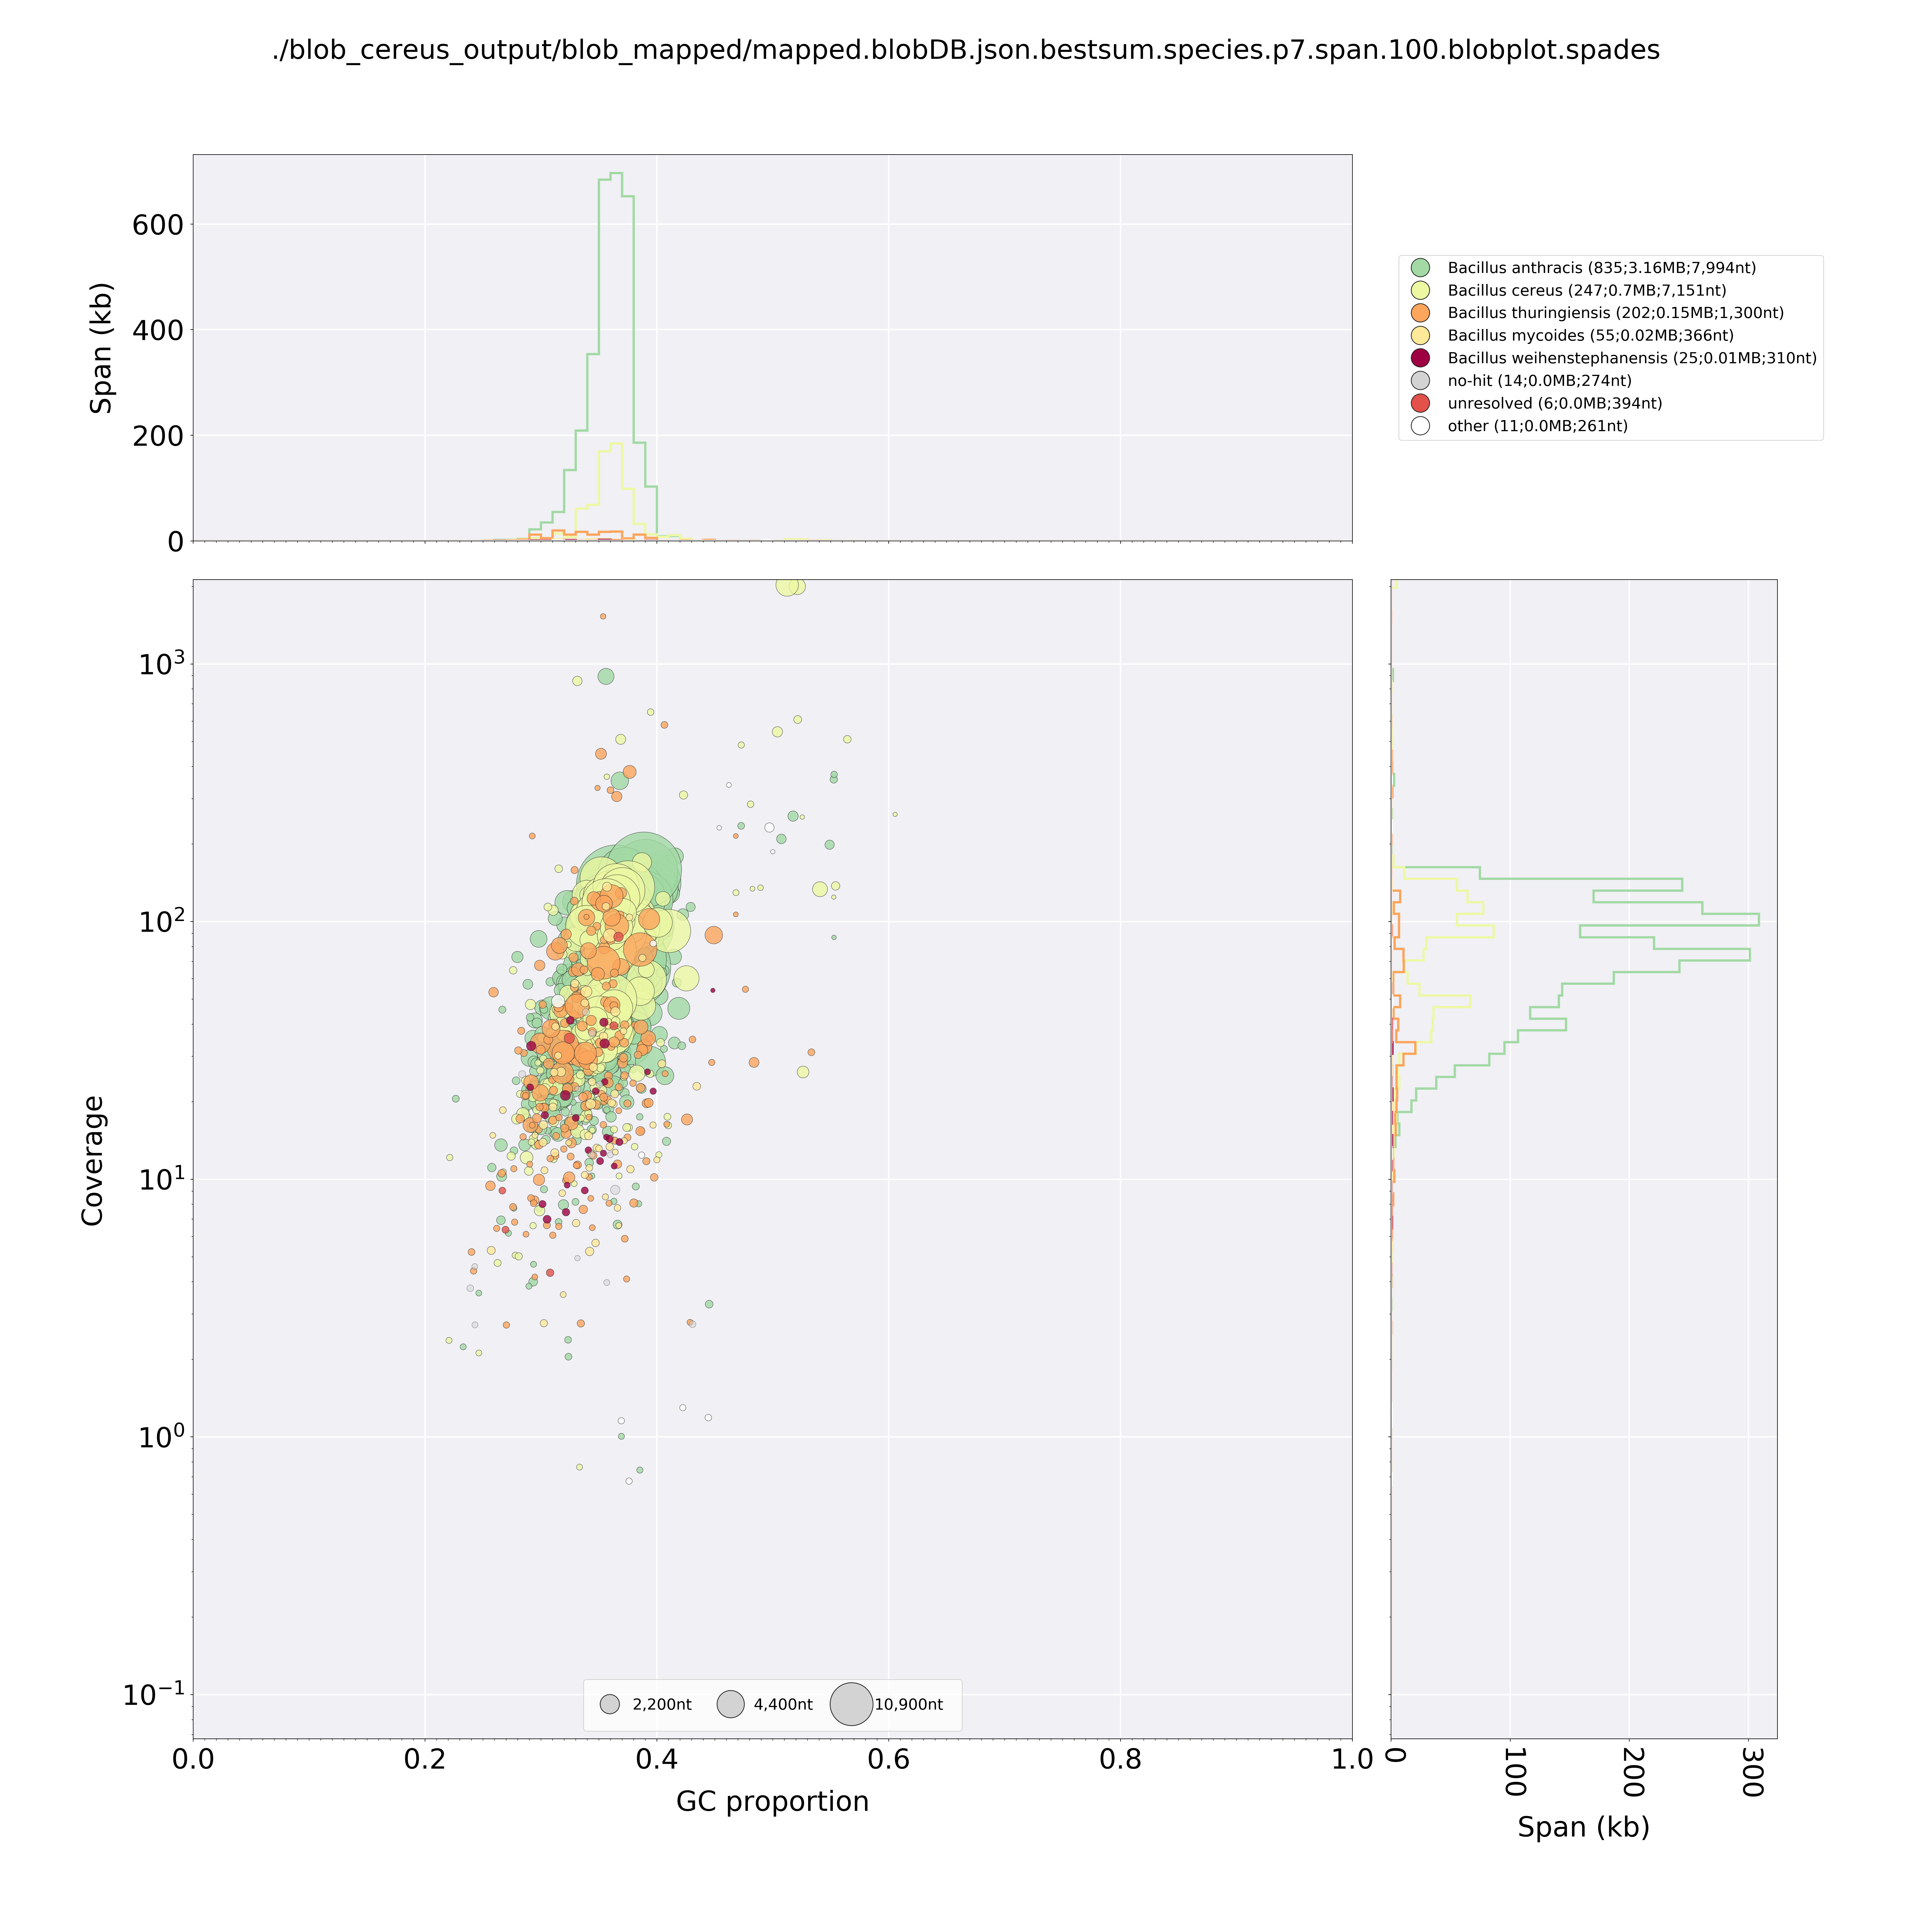
\includegraphics[width=.95\textwidth]{mapped.blobDB.json.bestsum.species.p7.span.100.blobplot.spades.png}
    \caption{Reads aligning to reference}
  \end{subfigure}
  \begin{subfigure}[b]{.5\textwidth}
    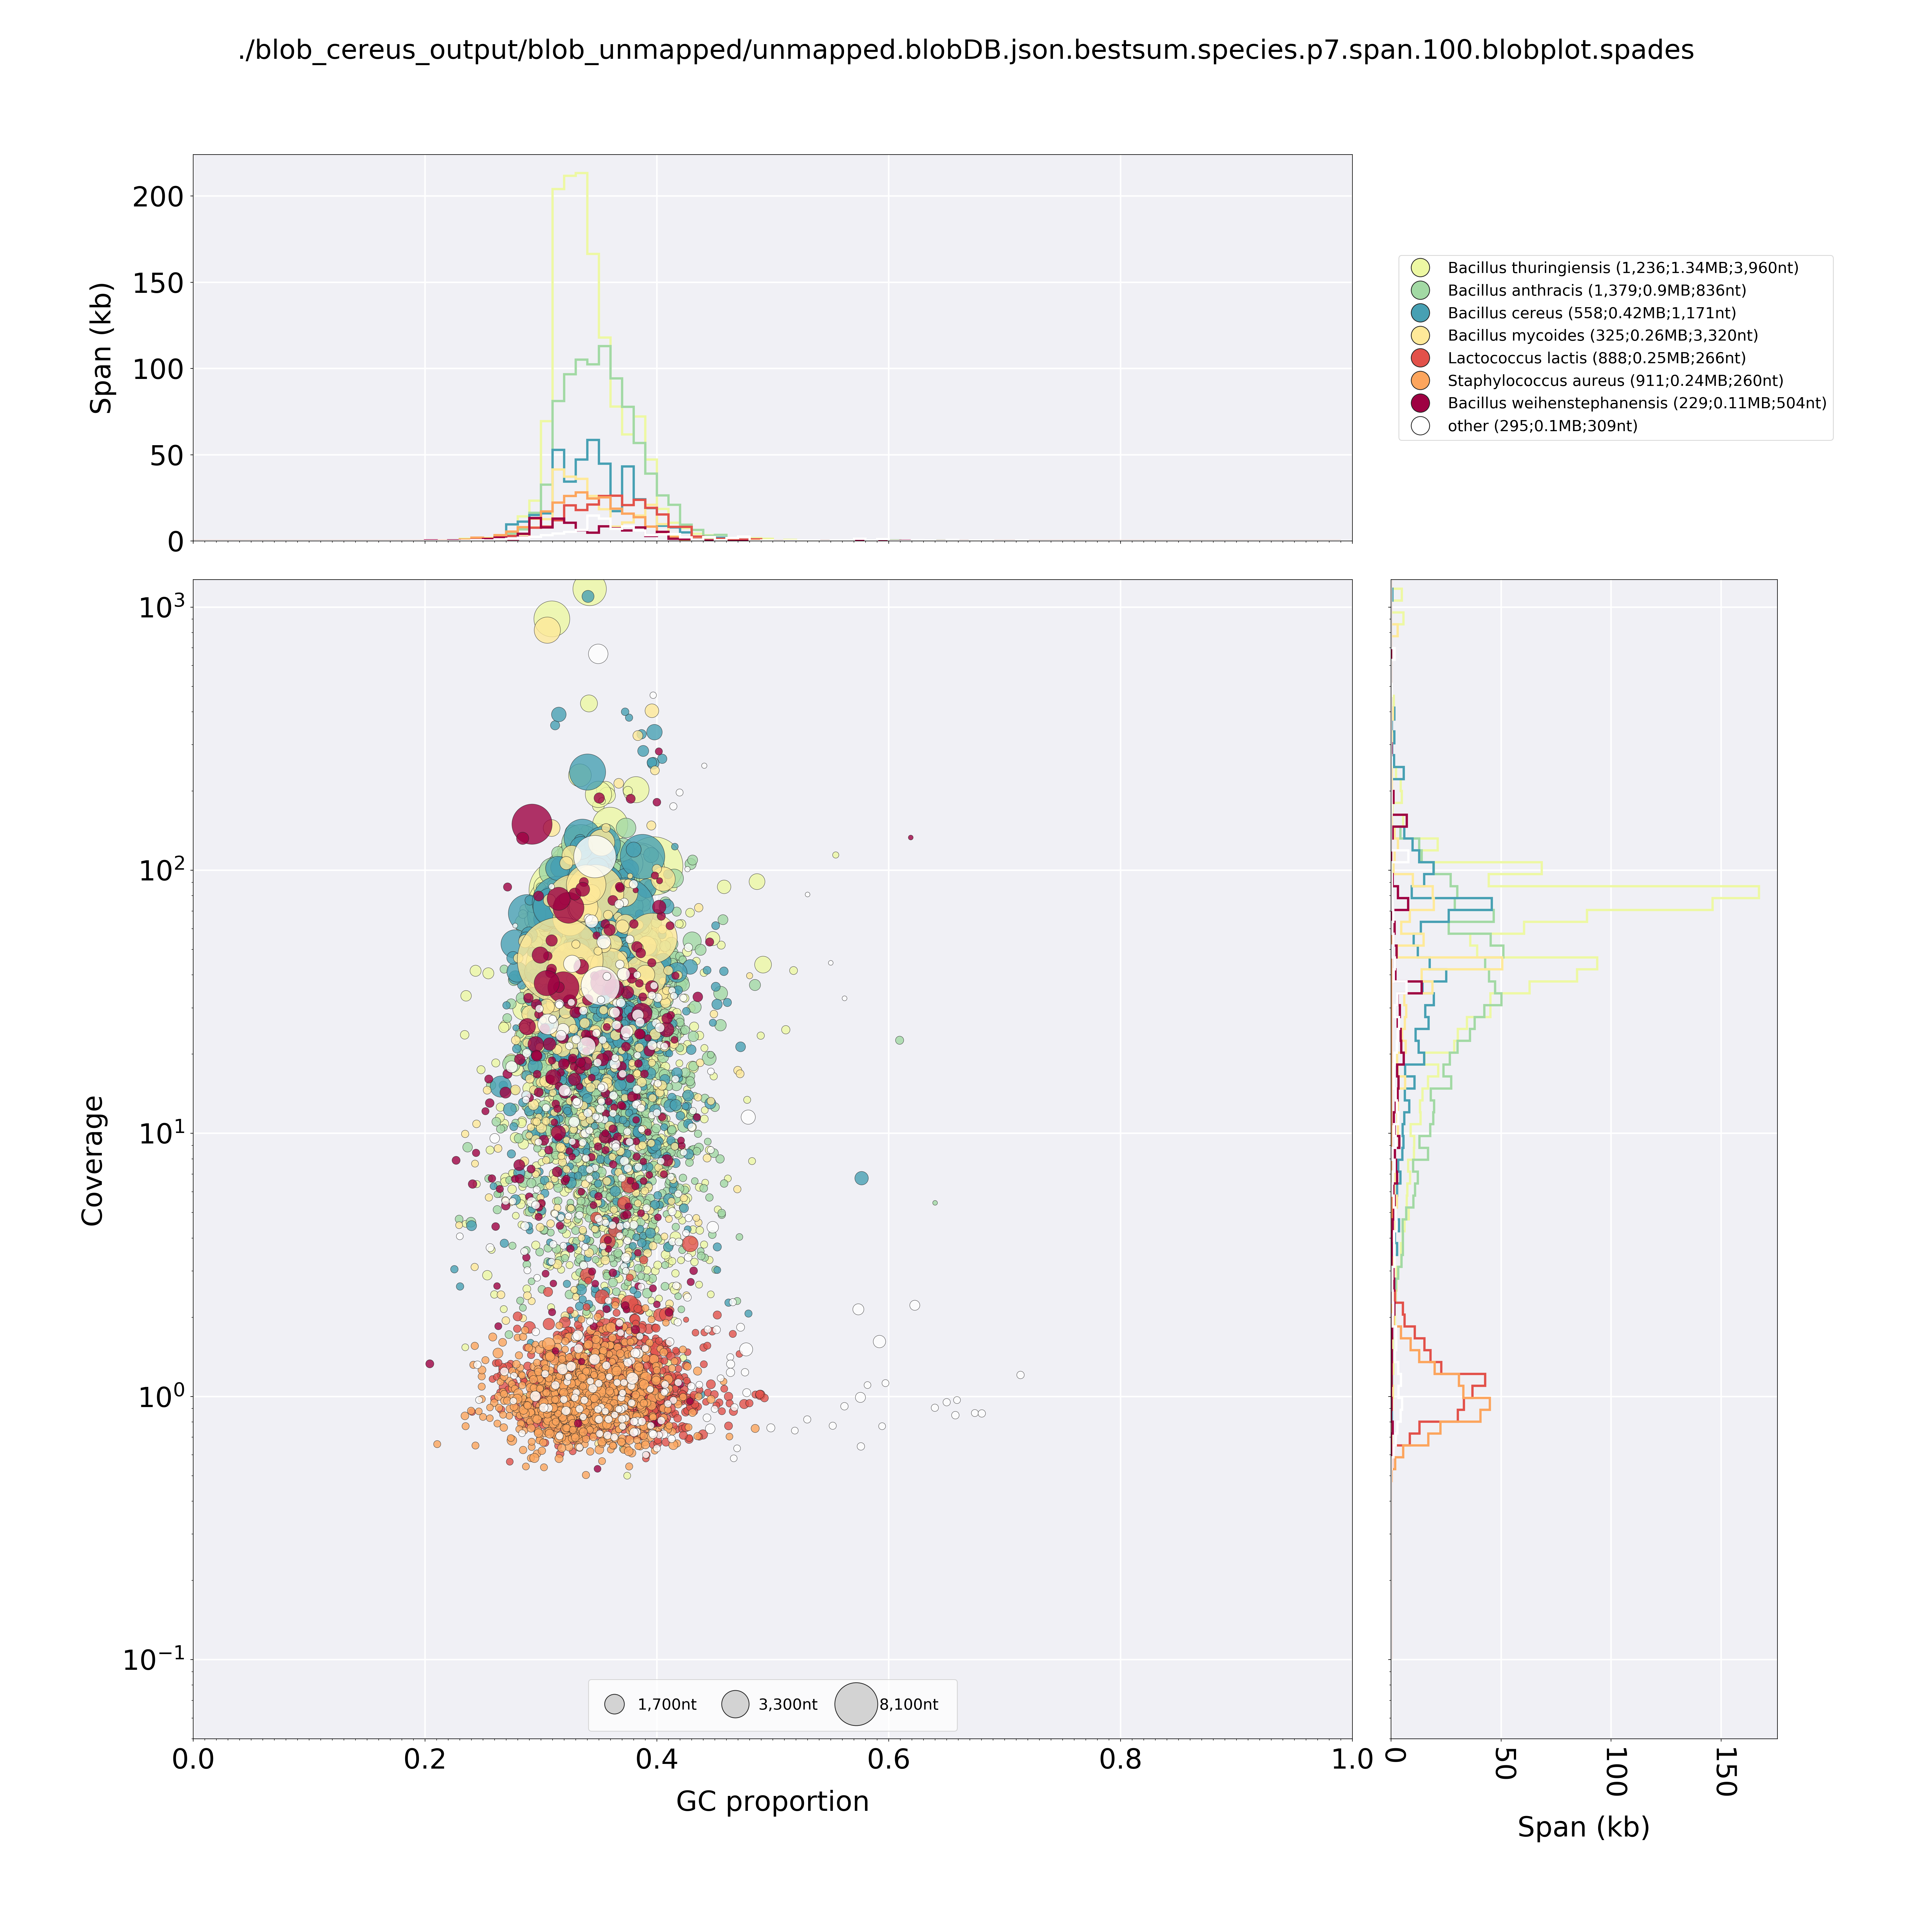
\includegraphics[width=.95\textwidth]{unmapped.blobDB.json.bestsum.species.p7.span.100.blobplot.spades.png}
    \caption{Reads failing to align to reference}
  \end{subfigure}
  \caption{Assessing contamination in the GAGE-B HiSeq \textit{B. cereus} dataset with blobtools. Reads were assembled with metaSPAdes, taxanomically assigned with BLASTn against the nt database, and plotted with blobtools.  (A) shows the whole dataset, while (B) and (C) shows the portion of the reads aligning to the \textit{B. cereus} ATCC 10987 reference and those failing to align, respectively.}
  \label{fig:contamination_all}
\end{figure}

The GAGE-B paper \cite{Magoc2013} notes that the \textit{B. cereus} HiSeq dataset proved particularly difficult to assemble. After noticing this irregularity, we re-assembled the trimmed reads downloaded from the GAGE-B website with metaSPAdes \cite{Nurk2017}  using default parameters.  Then, blastn was used to search the resulting contigs against NCBI's nt database (May, 2017) to get a list of hits according to the blobtools \cite{Laetsch2017a} specifications. Blobtools was then used to plot the hit coverage, taxonomy, and GC-content of the contigs.  This revealed what appears to be a contamination. \ref{fig:contamination_all}A. As the GC content of the contaminating organisms did not differ from \textit{B. cereus}, we believe that many tools that use GC-skew to detect contamination would not have detected the problem with this dataset.


To further show the contamination, we split reads into those read pairs mapping to the \textit{B. cereus} ATCC 10987 reference genome and those unmapped.  BWA MEM \cite{Li2013} was used to map the 12039737 reads to the reference genome;  samtools was used to separate the 7500534 reads (62\%) that mapped from the 3984200 reads (33\%) that failed to map with default parameters\footnote{The remaining \ttilde5 \% are those pairs where only one read aligned to the reference; these were ignored for this analysis.}.Each of these sets of reads was then assembled, BLASTed against the nt database, and plotted with blobtools \ref{fig:contamination_all}B and C.


Further, MaxBin \cite{Wu2014}, Kraken, and MBBC \cite{Wang2011} also supported the hypothesis that the sample is contaminated with approximately one third of reads originating from a non-\textit{B. cereus} strain.
